\subsection{Incremental SLAM and Loop Closure}

To evaluate the performance of Cartographer, we ran it using the 2012-11-16 run of the NCLT dataset as input. Plots are of the trajectory from the 11 to 13 minute mark from the start of the dataset. The provided ground truth, odometry, and Cartographer operating in 2D and 3D mode are compared. Note that this section evaluates error over a 2 minute long loop, rather than 20 seconds of operation while turning.

We found that for our dataset, we had to assign a high weight to rotation and translation changes in the optimizer, exactly two orders of magnitude greater than the default settings. Higher weights correspond to increased trust in the prior provided by IMU and odometry measurements, meaning that the result of scan-to-submap matching was more likely to introduce error to the output trajectory than the odometry and IMU priors.

Compared to the trajectory smoothing and InEKF approaches, Cartographer's scan-to-submap matching accumulates an order of magnitude less error over 2 minutes than the incremental methods accumulate over 20 seconds. See Table \ref{tb:cartographer-3d-error-table}, Table \ref{tb:cartographer-2d-error-table}, and Table \ref{tb:Error_Table}. However, there is a significant amount of z-axis drift introduced when running Cartographer in 3D mode. This drift is corrected by global optimization at the 56 and 84 second marks, but z-axis error continues to accumulate at about 2 meters per minute. This can be partially remedied by locking the roll and pitch during scan matching, which we have done, but without another method of minimizing z-axis error, it will accumulate enough to prevent larger loops from being closed. Alternatively, additional sensors can be integrated into the optimization problem to correct z-axis error. The Segway also includes data from two Hokuyo lidars, one mounted in a push-broom configuration facing the ground and the other mounted facing forward. The ground-facing lidar could be incorporated into the scan matching algorithm so that tracking the ground is incorporated into the algorithm. Finally, altitude estimates could be integrated from one of the GPS receivers as fixed-frame reference points.

While 2D mode was not prone to accumulating z-axis drift like 3D mode, it was significantly more likely to experience runtime errors (segfaults and assertion failures). Most of Cartographer's development has been focused on optimizing for the 3D use-case, so it's likely that these bugs have gone unnoticed because most applications use the 3D trajectory builder interface.

\begin{table}[h]
	\captionsetup[table]{position=here}
    \caption{\label{tb:cartographer-3d-error-table}
    3D Error Analysis using Cartographer
    }
    \begin{center}
    \resizebox{\linewidth}{!}{
        \begin{tabular}{c | *2{c}}
			\toprule
            Dataset & Mean 3D Pose Error (m) & End 3D Pose Error (m) \\
            \hline
             Odometry Only & 1.09 & 1.73 \\
             Cartographer 3D & 3.16 & 7.34 \\
             Cartographer 2D & 1.87 & 4.97 \\
			\bottomrule
        \end{tabular}}
    \end{center}
\end{table}

\begin{table}[h]
	\captionsetup[table]{position=here}
    \caption{\label{tb:cartographer-2d-error-table}
    2D Error Analysis using Cartographer
    }
    \begin{center}
    \resizebox{\linewidth}{!}{
        \begin{tabular}{c | *2{c}}
			\toprule
            Dataset & Mean 2D Pose Error (m) & End 2D Pose Error (m) \\
            \hline
             Odometry Only & 1.06 & 1.69 \\
             Cartographer 3D & 2.02 & 5.89 \\
             Cartographer 2D & 1.85 & 4.96 \\
			\bottomrule
        \end{tabular}}
    \end{center}
\end{table}

\begin{figure}[hbt!]
    \centering
    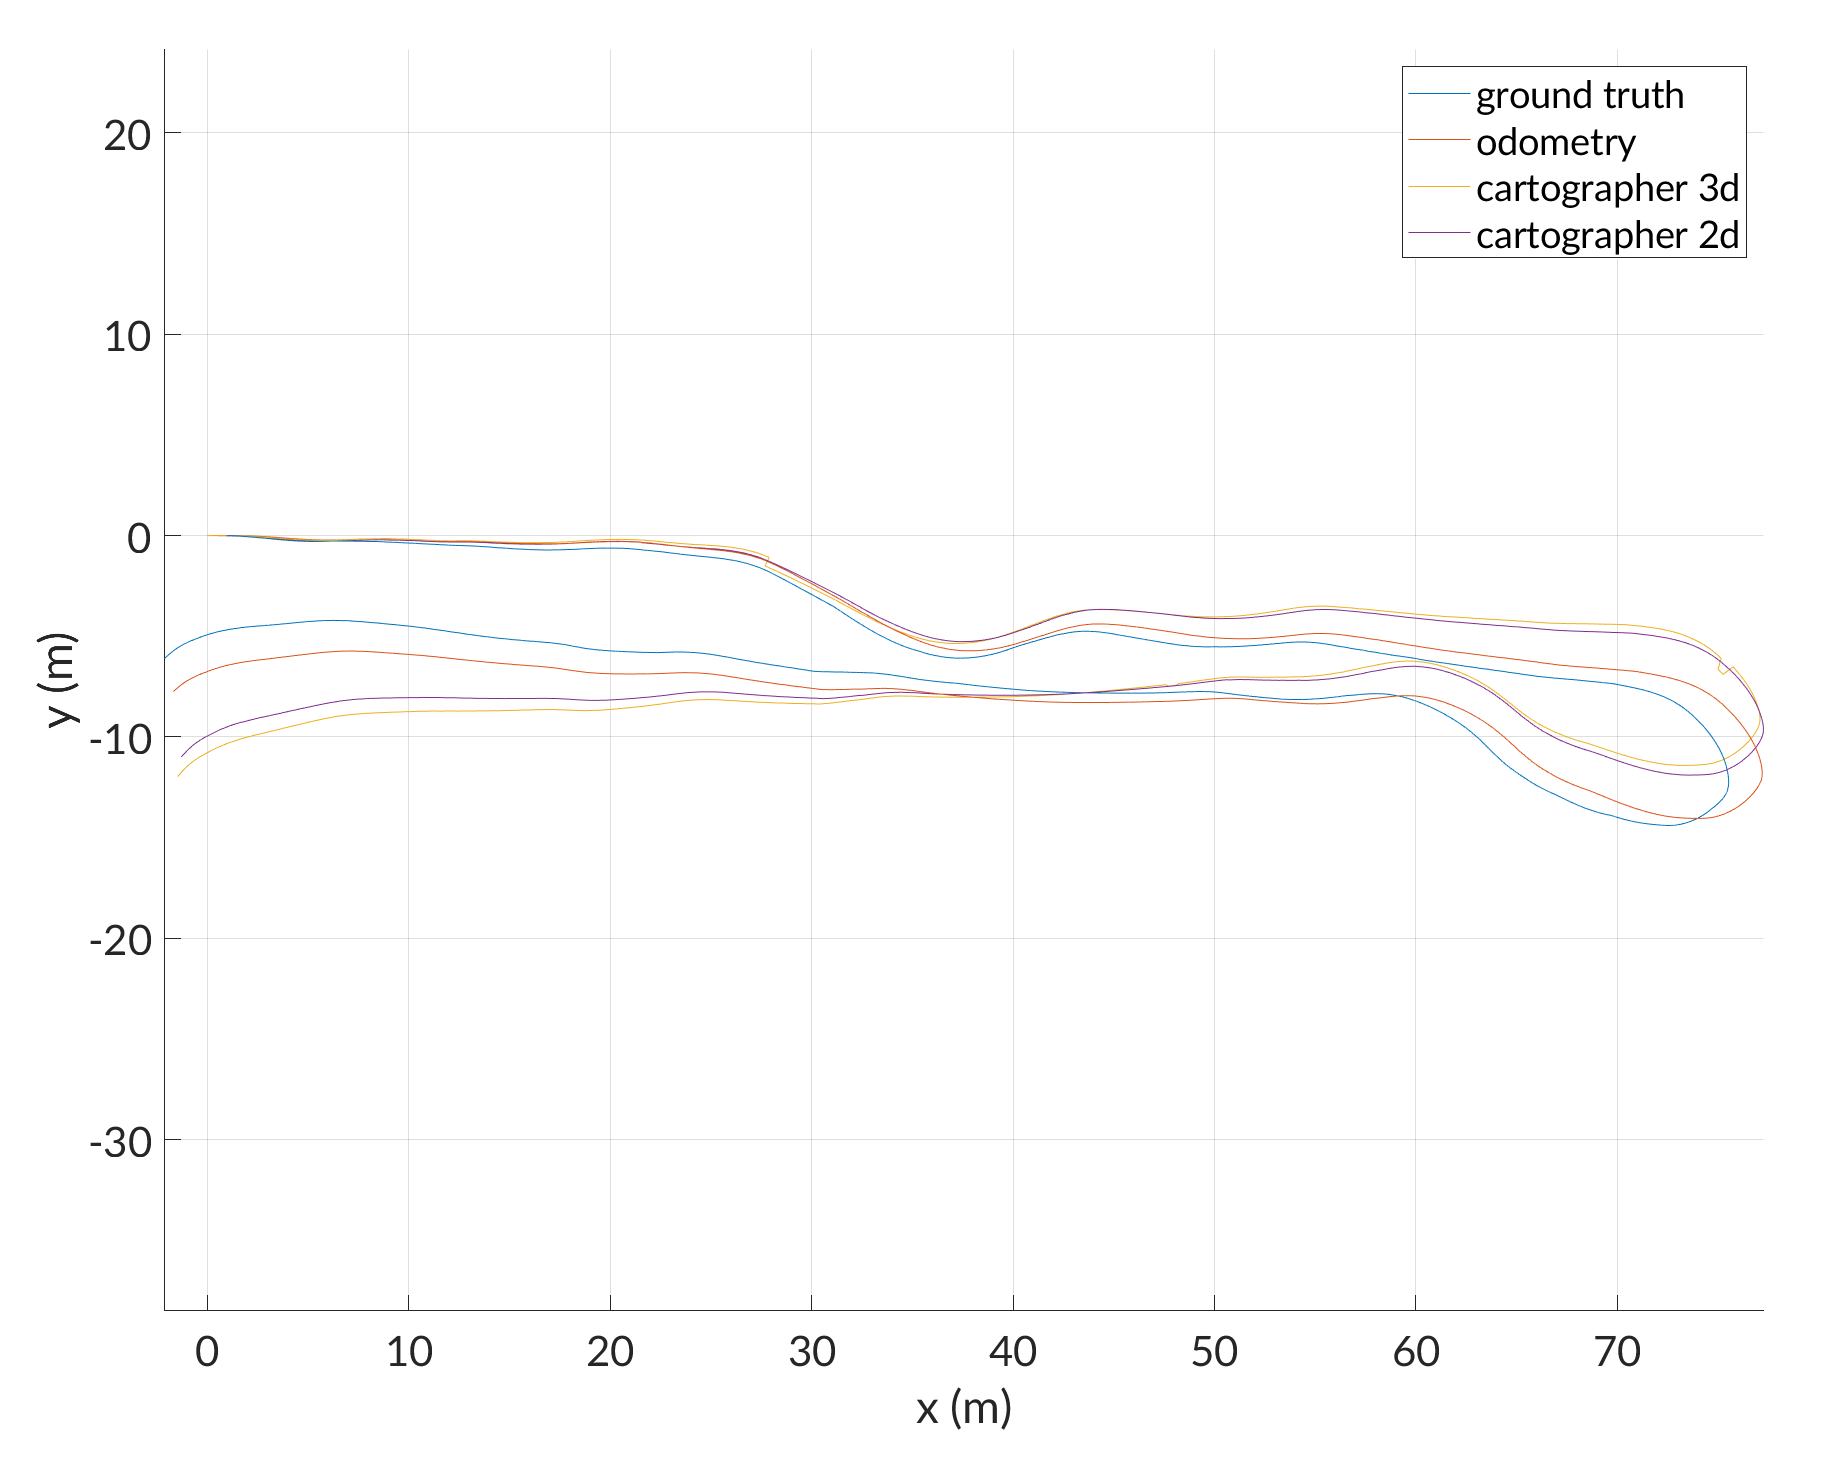
\includegraphics[width = 0.8\linewidth]{media/cartographer/error-top.png}
    \caption{\textit{x-y view of optimized trajectories.}}
    \label{fig:cartographer-xy}
\end{figure}

\begin{figure}[hbt!]
    \centering
    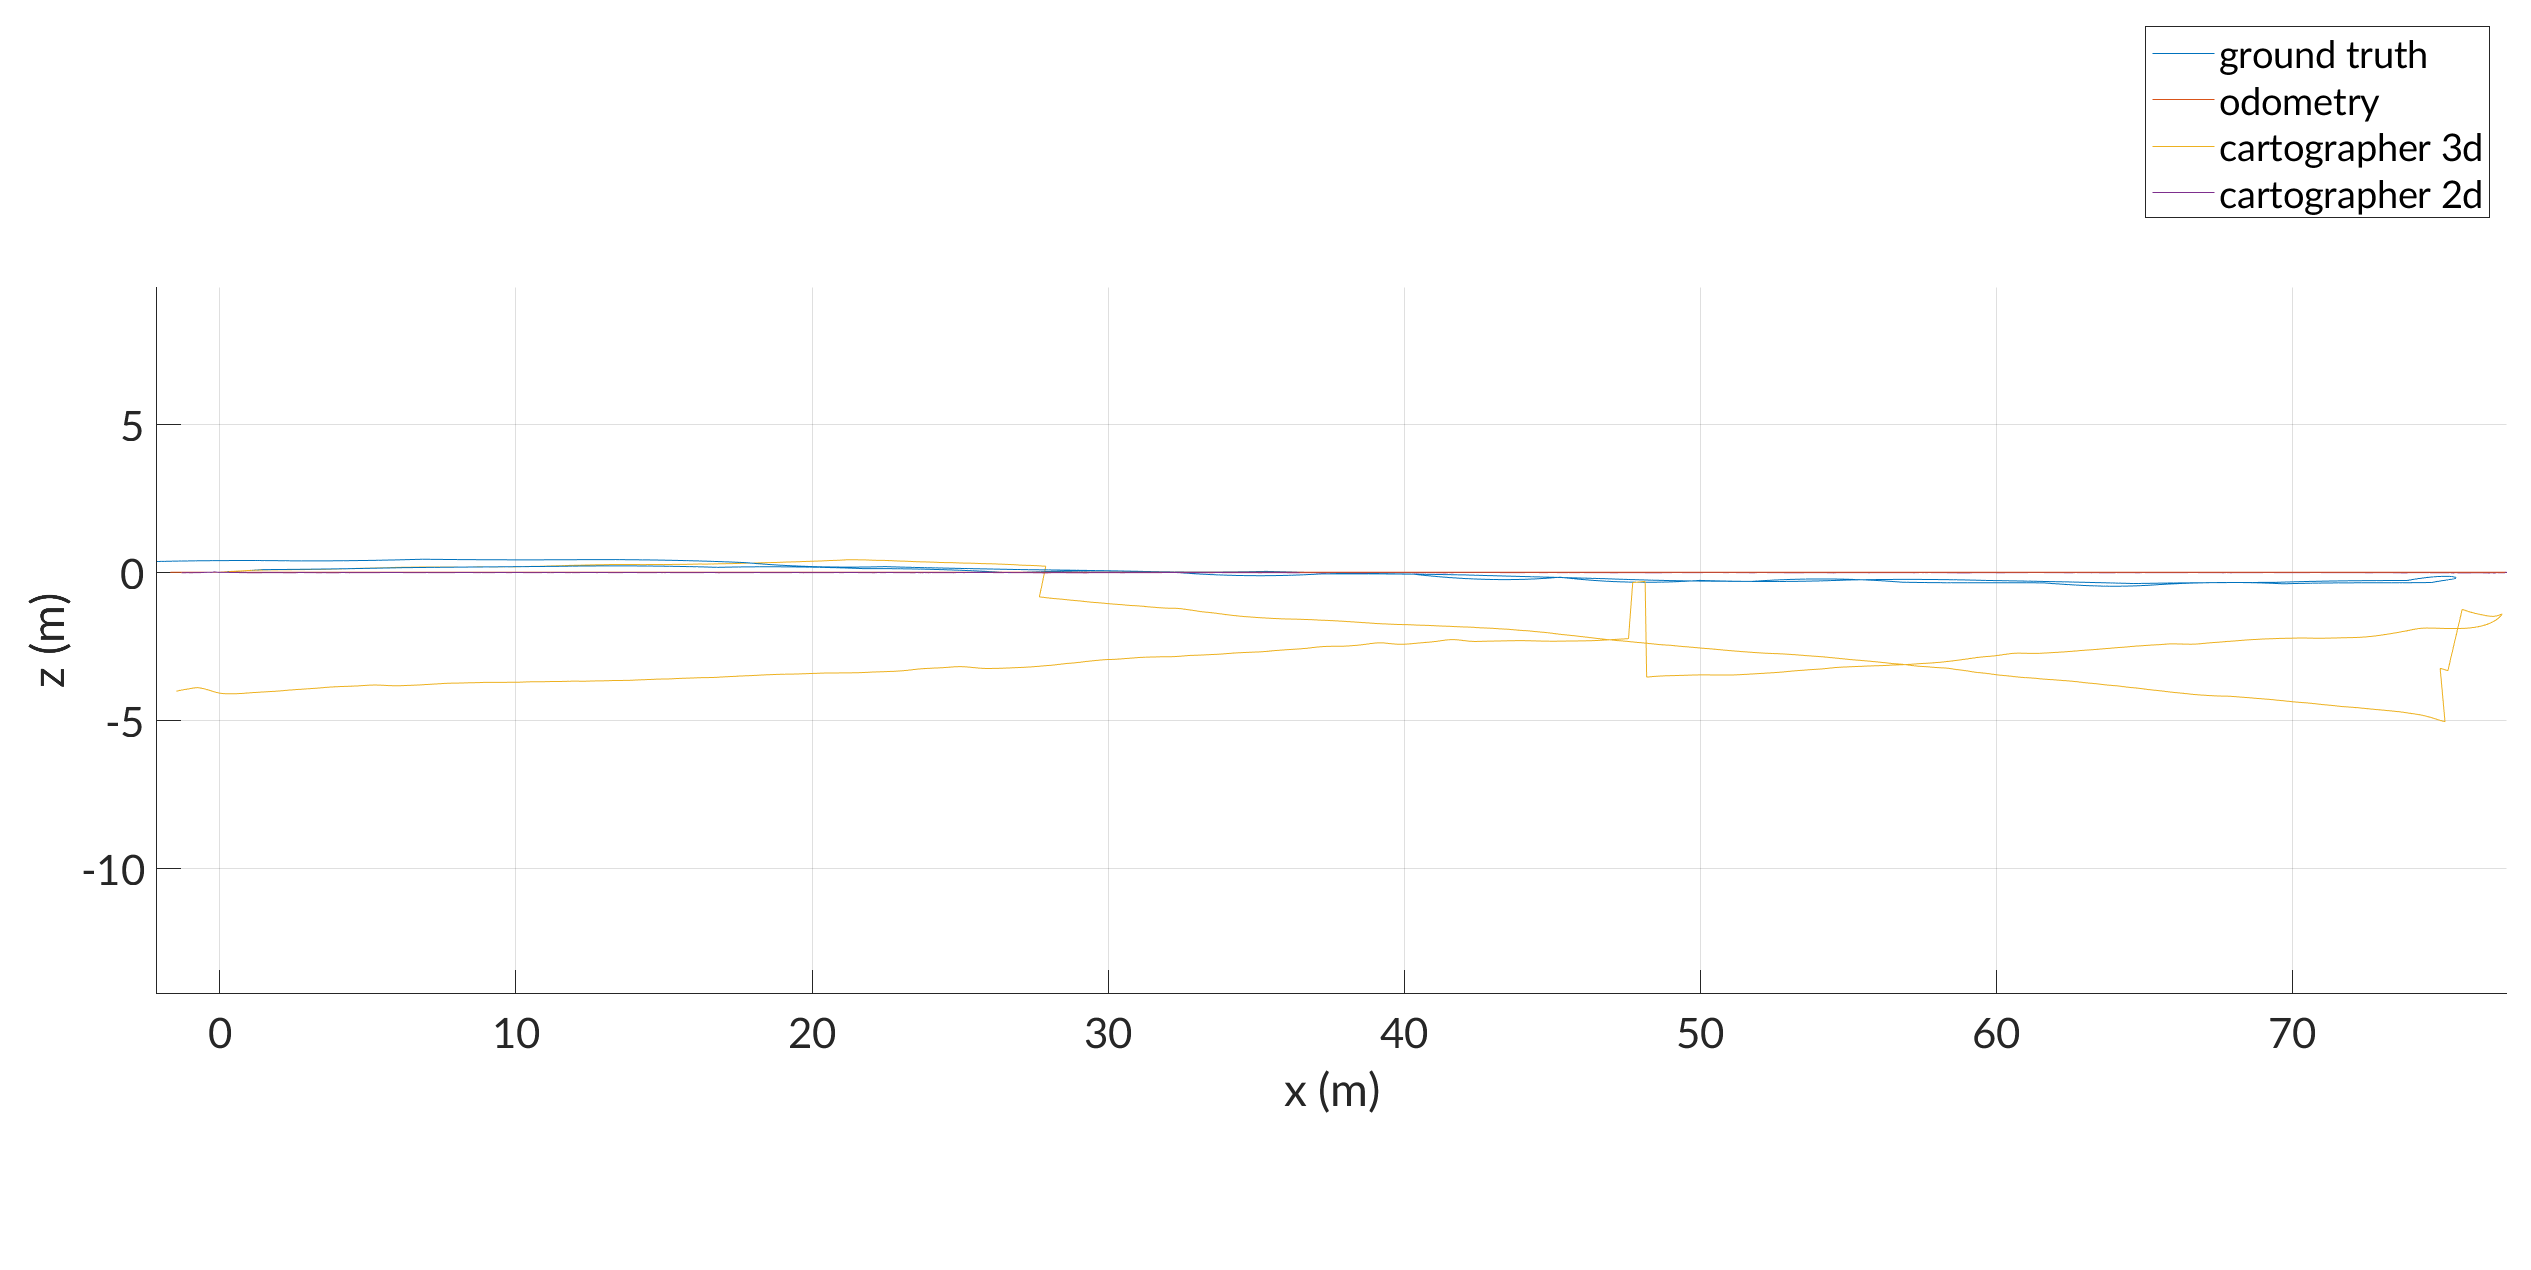
\includegraphics[width = 0.8\linewidth]{media/cartographer/error-side.png}
    \caption{\textit{x-z view of optimized trajectories.}}
    \label{fig:cartographer-xz}
\end{figure}

\begin{figure}[hbt!]
    \centering
    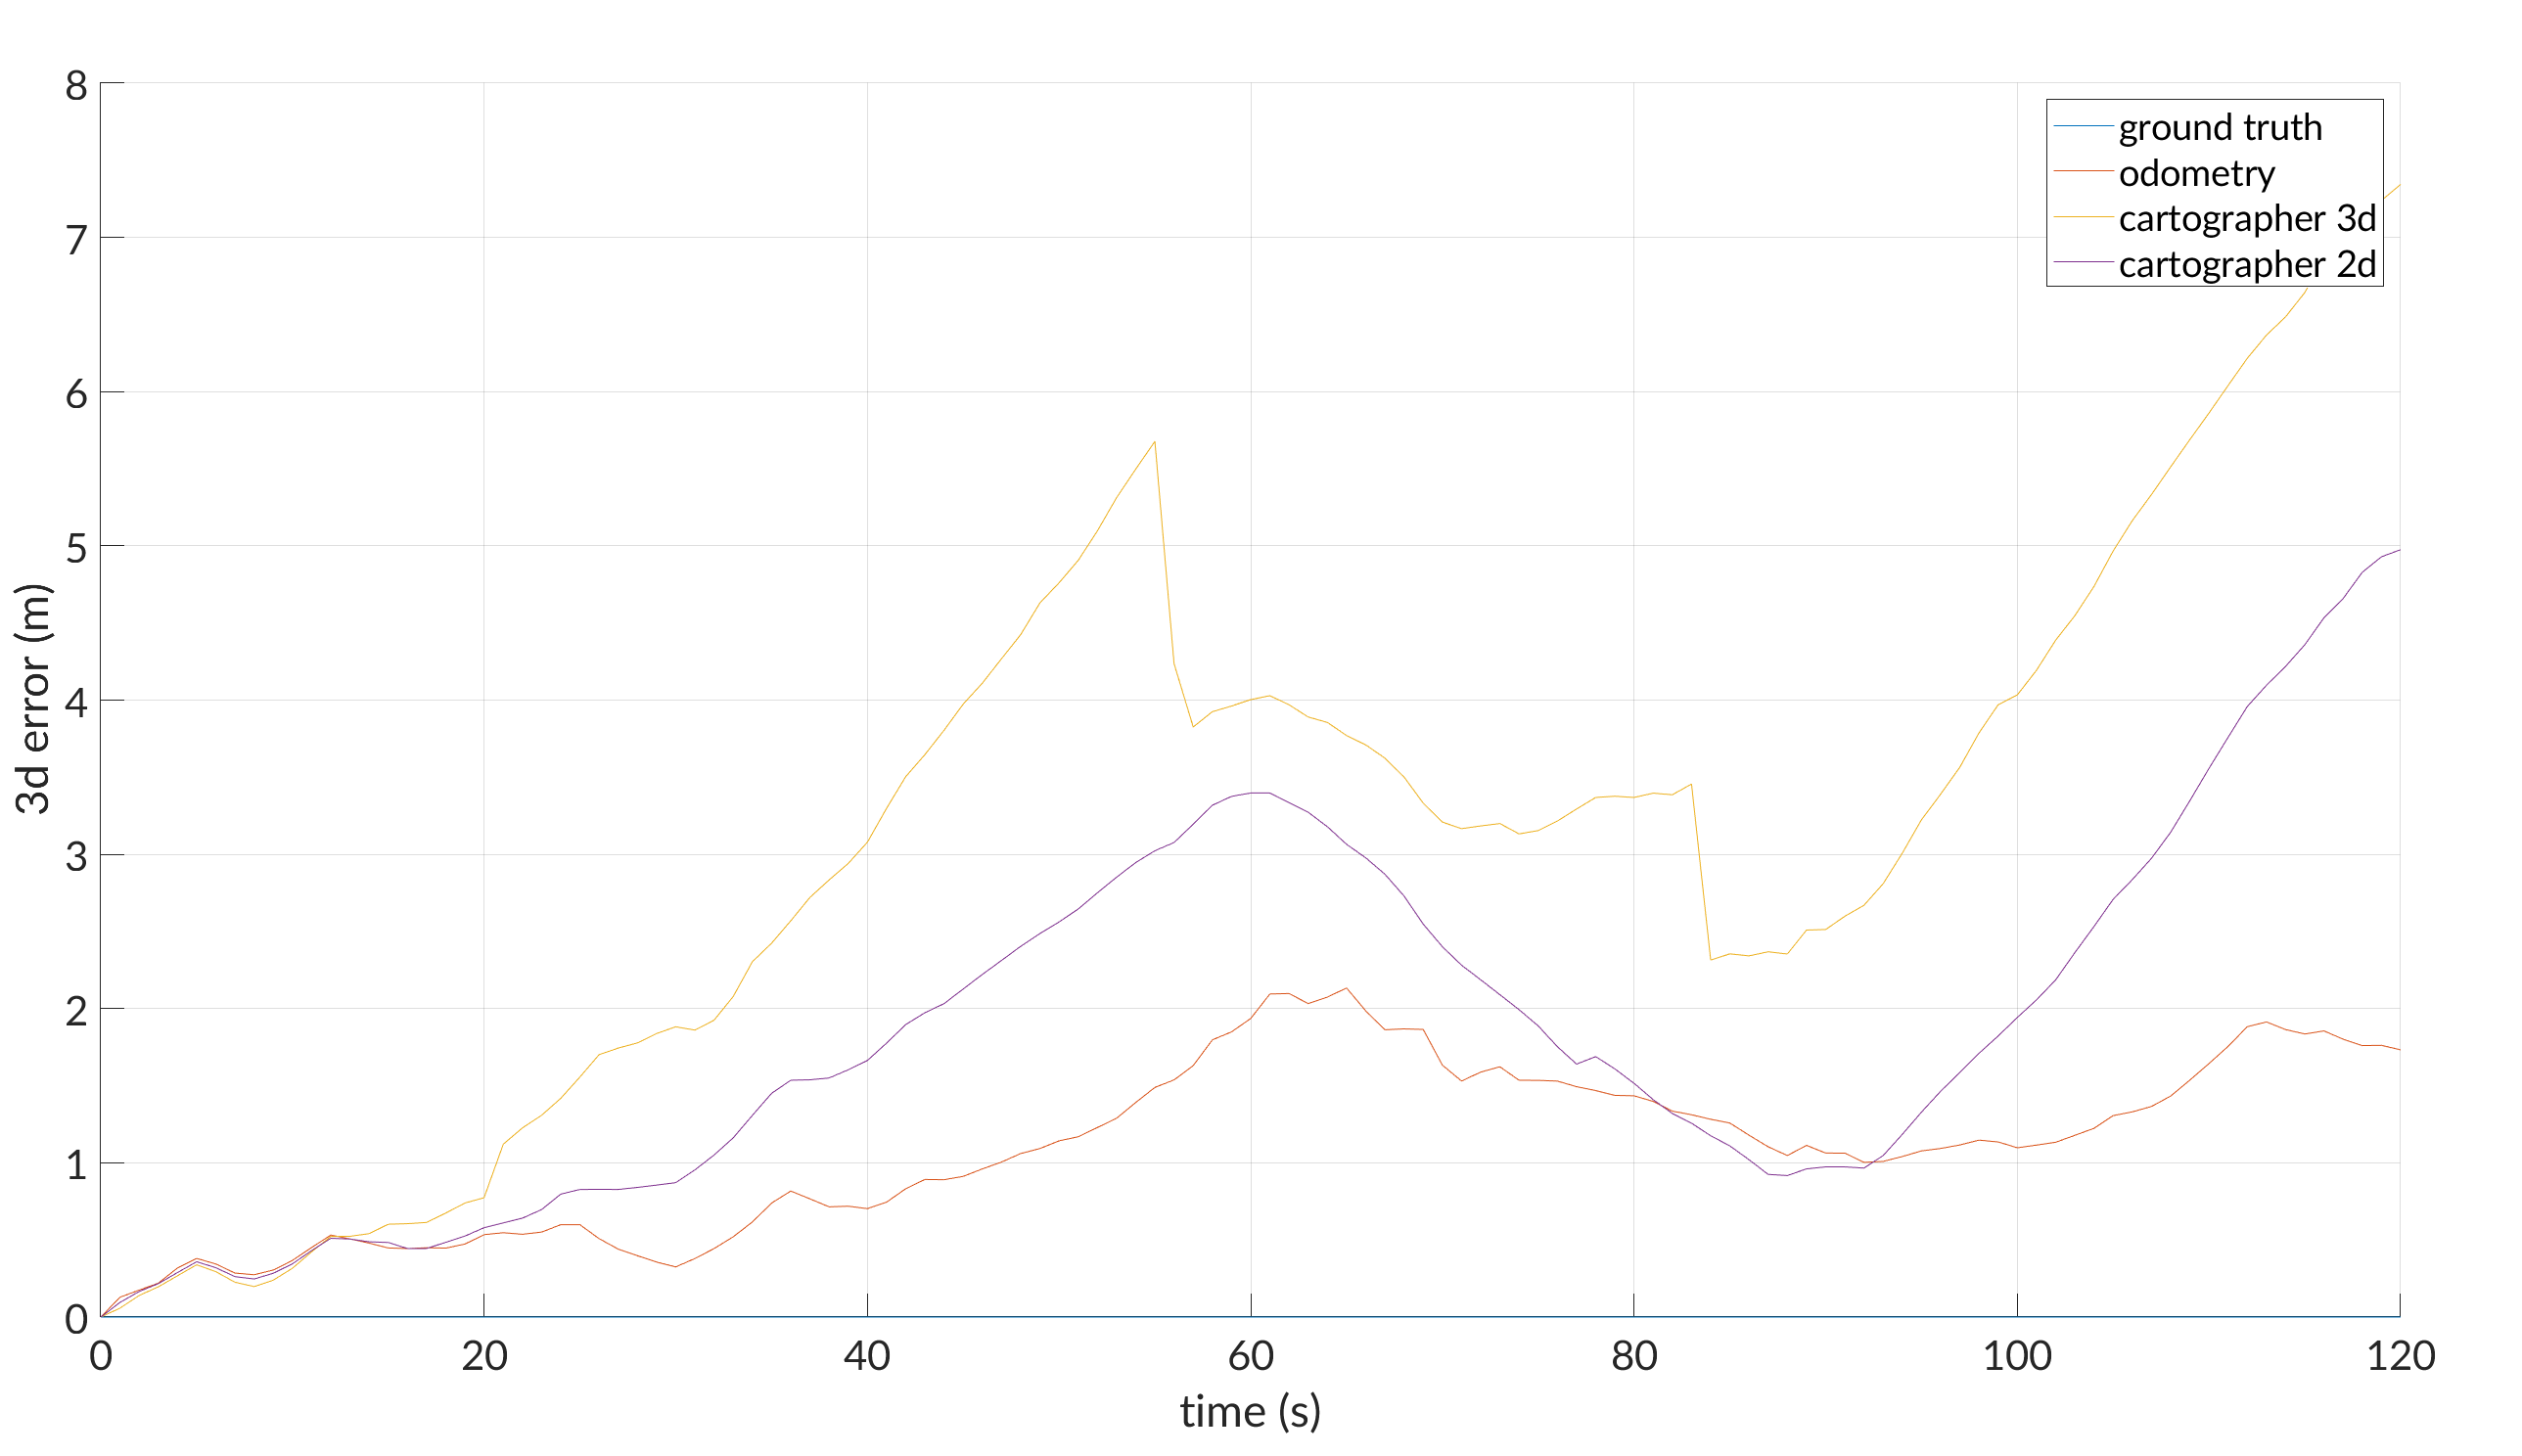
\includegraphics[width = 0.8\linewidth]{media/cartographer/3d-translation-error.png}
    \caption{\textit{3D translation error.}}
    \label{fig:cartographer-3d-error}
\end{figure}

\begin{figure}[hbt!]
    \centering
    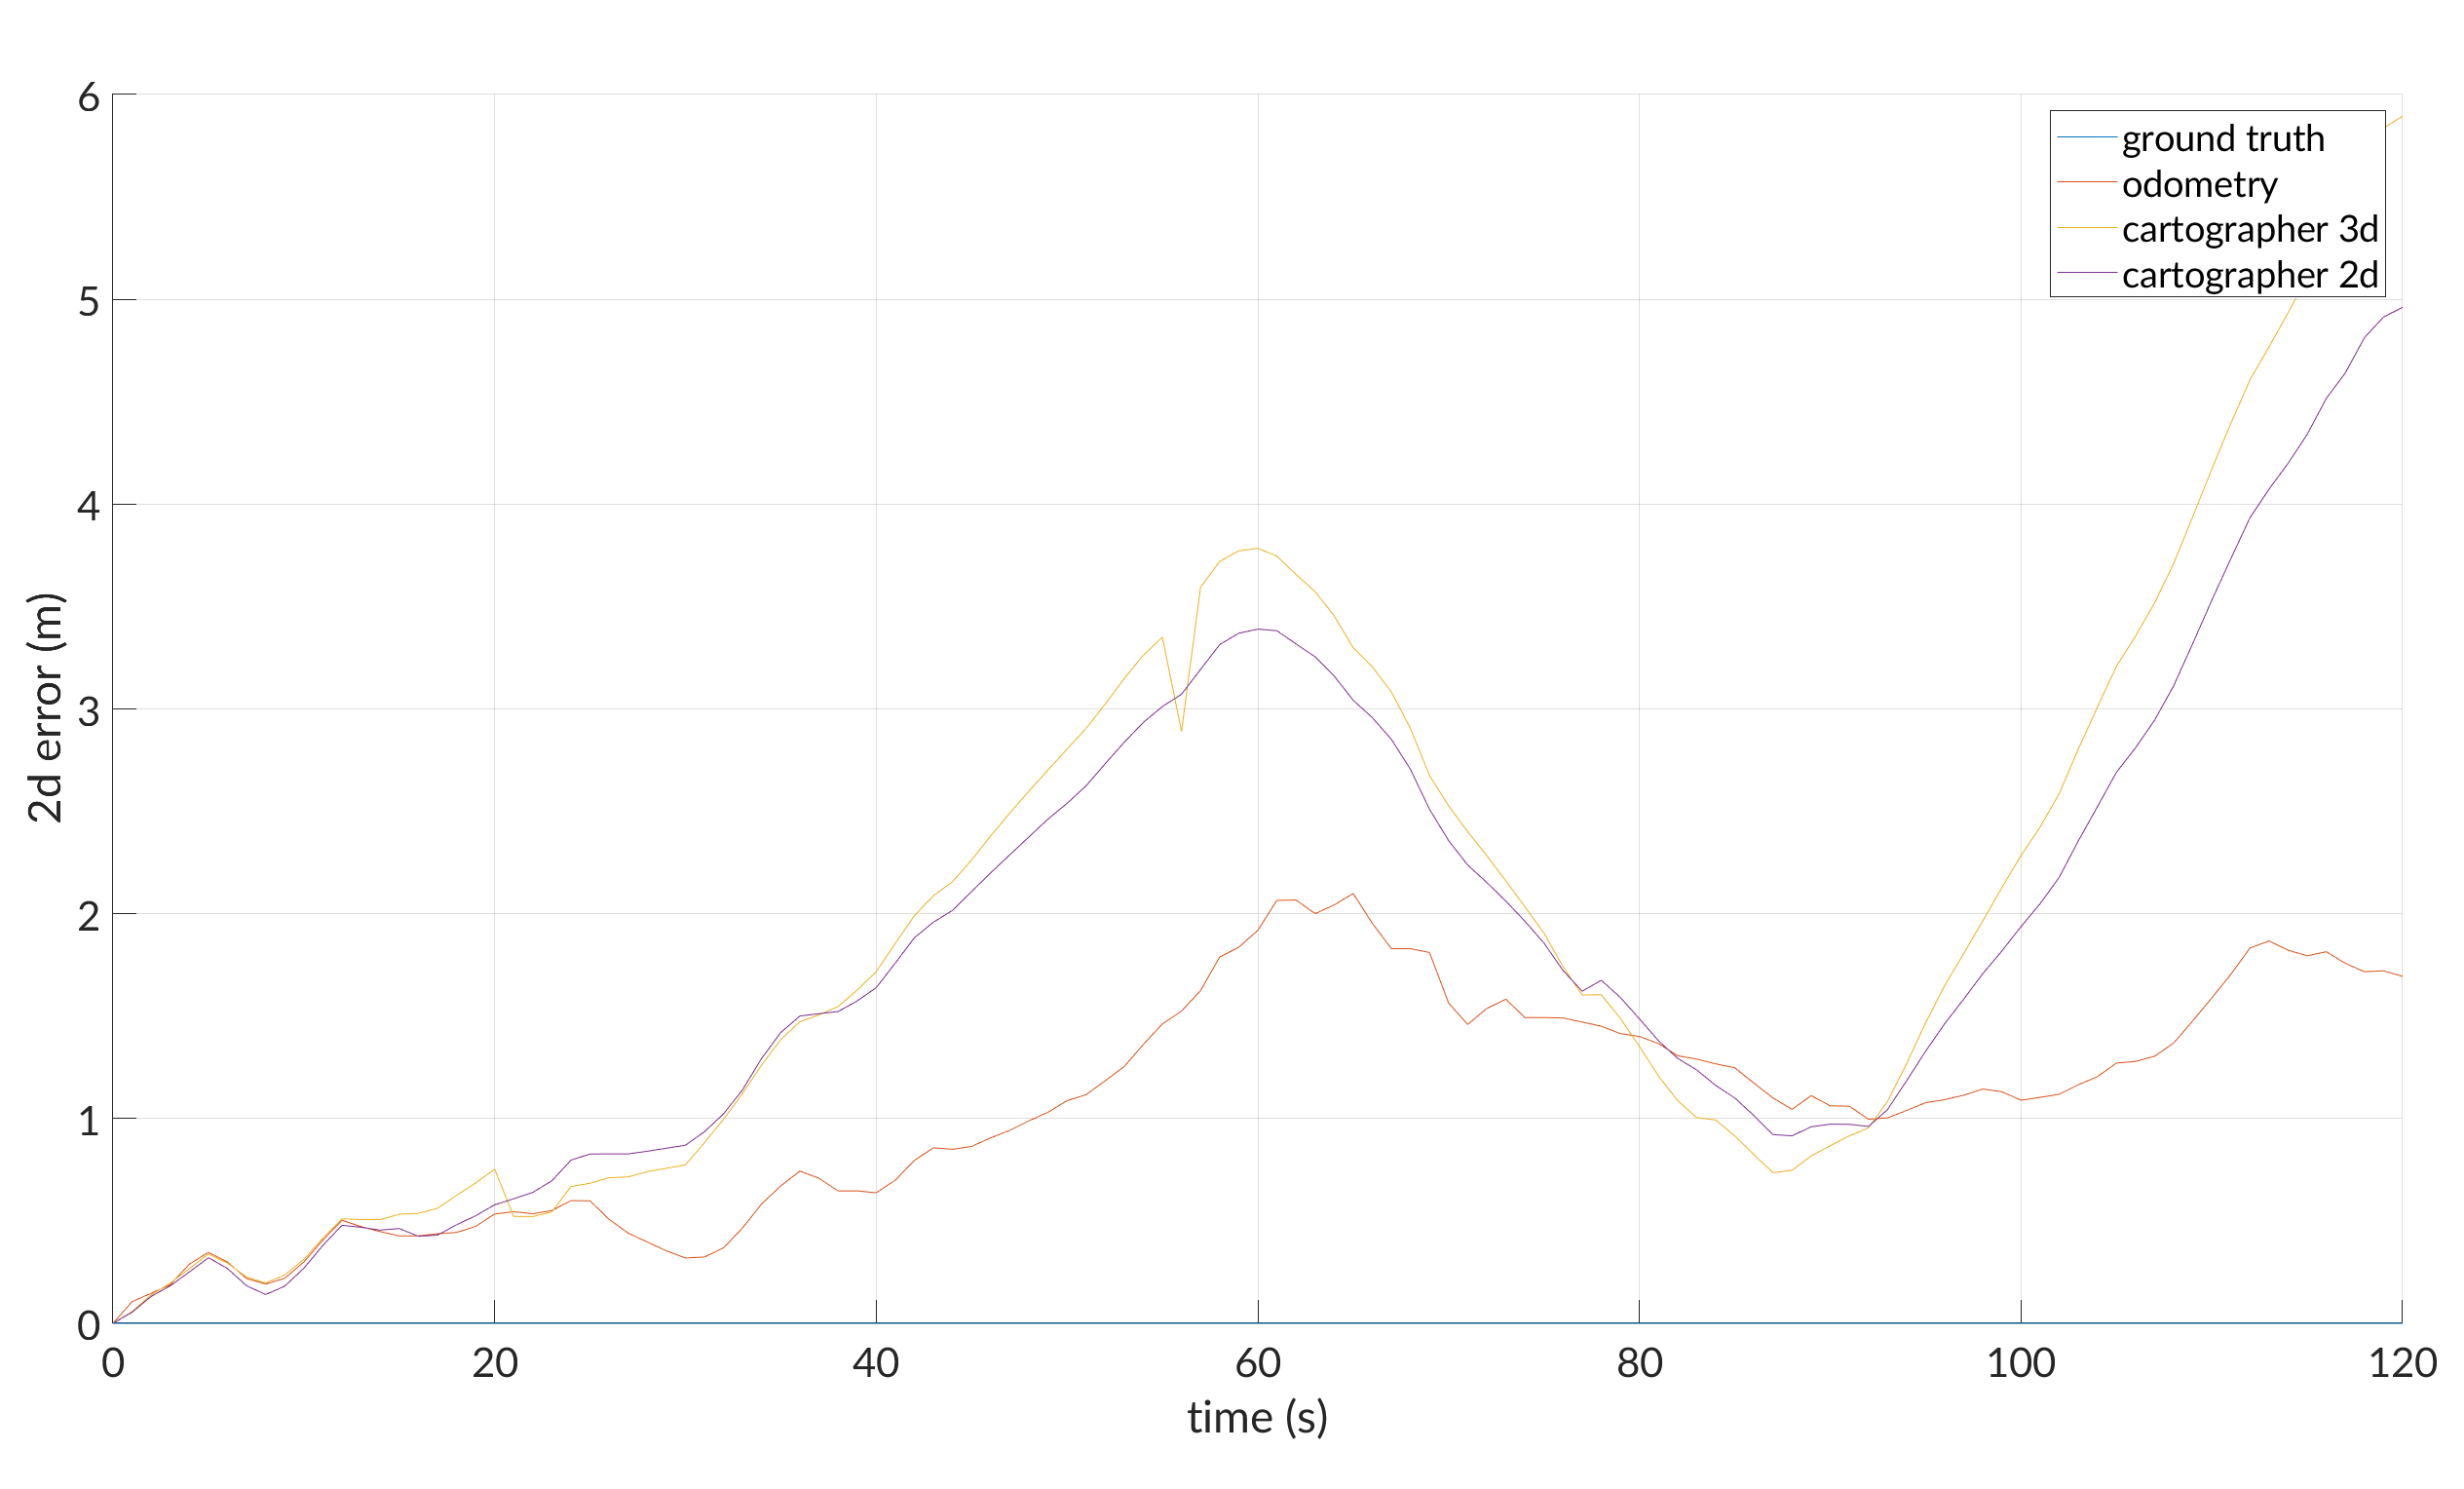
\includegraphics[width = 0.8\linewidth]{media/cartographer/2d-translation-error.png}
    \caption{\textit{2D translation error.}}
    \label{fig:cartographer-2d-error}
\end{figure}

\subsection{Trajectory Smoothing Analysis}
This section includes the error analysis of trajectory smoothing. The main concentration is on mean error,  end pose error and covariance. Mean error in Table. \ref{tb:Error_Table} represents average mean error in meter at each individual step. End pose error refers to the distance error which is equal to $location_{real}(x,y) - location_{ground truth}(x,y)$ Covariance is the covariance between ground truth position and the estimated position. The detail is given in Table. \ref{tb:Error_Table}.

\begin{table}[h]
	\captionsetup[table]{position=here}
    \caption{\label{tb:Error_Table}
    Error Analysis using Trajectory smoothing
    } 
    \begin{center}
    \resizebox{\linewidth}{!}{
        \begin{tabular}{c | *3{c}}
			\toprule
            Dataset & Mean Error(m) & Average Covariance(m\textsuperscript{2}) & End Pose Error(m) \\
            \hline
             $Odometry+Gyro$ & 116.43 & 13783.43 & 154.53  \\
             $Gyrodometry$ & 125.75 & 16482.48 & 178.49 \\
             $GPS+IMU$ & 21.41 & 459.02 &79.94 \\
             $GPS+Odometry$ & 9.14 & 92.41 & 75.95 \\
			\bottomrule
        \end{tabular}}
    \end{center}
\end{table}

\subsubsection{Analysis about odometry Data}
Theoretically, gyrodometry should perform better result than pure odometry and odometry + Gyro data. However, Table.\ref{tb:Error_Table} and Figure.\ref{fig:Gyrodometry} show that ``gyro-only" correction methods beats other odometry correction methods. One of the explanation is that the gyro sensor(KVH DSP-3000 single-axis FOG) in NCLT dataset provides highly accurate rotation measurements. Moreover, the gyro data  biased towards the same side as the odometry data, thus gyro cannot aid the correction of the trajectory a lot.

Additionally, even though the shape of the trajectory looks similar to the ground truth, the error accumulates through the entire trajectory, because there is no sensor measurement for correction. Thus, simply using odometry + Gyro data is not ideal method. The next section brings GPS data into discussion for minimizing the bias of the trajectory. 

\subsubsection{Analysis about GPS Data}
From Figure. \ref{fig:IMU-GPS}, as the GPS data obtained is noisy, lots of overshoots exist in the trajectory. To correct the overshot portion of the trajectory, GPS is preferred to be filtered with IMU data. 

With ISAM2 method, the overshoots can be minimized and filter GPS trajectory can be viewed in Figure. \ref{fig:filteredgps}. To tune a better trajectory, IMU variance value is to set high($\sigma_{angular}$ = 10) on angular direction. Although the filtered GPS trajectory seems to be closer to the ground truth from Table. \ref{tb:Error_Table} and the orientation of the trajectory is about to align with the ground truth, the details of the trajectory is not good enough as the trajectory estimation. Then, to further corrects the trajectory, combing with corrected odometry data would be preferred. 

\subsubsection{Analysis about GPS + Odometry Data}
The filtered Odometry data are used to create graph and filted GPS data are added as factors such that by tuning the covariance values, the trajectory can be further optimized and obtained in Figure. \ref{fig:Final plot}. The strategy to tune a better trajectory is to set sigma large($\sigma_{linear}$ = 100) on linear direction and set low sigma value ($\sigma_{angular}$ = 0.3) on angular direction.

Overall, the filtered data using modified odometry and modified GPS shows the best result among all method in Table. \ref{tb:Error_Table}. However, the filtered trajectory looks bad when the robot drives in a complicated manner shown in Figure \ref{fig:Final plot} (the details of the trajectory is messy). In contrast, the overall filtered trajectory is a good represent of the location of robot when it moves in a relatively simple minor, like driving in a straight line or doing some square movement. One of the possible reason is that the GPS is noisy when the robot performs continuous turning in a short amount of time such that the GPS data cannot be updated correctly.

% To do: edit the latex structure

\subsection{Left-InEKF Analysis}

This section examines the result from the Left-InEKF. By comparing the result with the given ground truth, error analysis is performed and presented in Table \ref{tb:Error_Table_2}.

\begin{table}[h]
	\captionsetup[table]{position=here}
    \caption{\label{tb:Error_Table_2}
    Error Analysis for Left-InEKF
    } 
    \begin{center}
    \resizebox{\linewidth}{!}{
        \begin{tabular}{c | *3{c}}
			\toprule
            Dataset & Mean Error(m) & Average Covariance(m\textsuperscript{2}) & End Pose Error(m) \\
            \hline
             $GPS+IMU InEKF$ & 95.32 & 8801.55 &109.94 \\
			\bottomrule
        \end{tabular}}
    \end{center}
\end{table}

In comparison with the trajectory smoothing output using GPS and IMU (Table \ref{tb:Error_Table}), the InEKF estimation has approximately 10\% larger error. As shown in Figure \ref{fig:complete_IMUGPS_result}, the estimation is the most accurate at the beginning of the data collection, starting at the origin. However, it gradually deviates away from the ground truth, despite of the general shapes of the two plots being similar. 

The error may have been caused by the following reasons. First, the covariance is not well tuned for the filter. If a larger sigma is assigned to the input and observation, a more accurate estimation will be obtained. Second, the GPS data is rather jumpy as shown in Figure \ref{fig:IMU-GPS}. If the GPS measurement is smoothed before inputting into the filter, the result could have been be better. In addition, the overall size of the estimated trajectory is larger than that of the ground truth, which indicates a probable system error in the calculation to transform the latitude and longitude to the x-y location. Lastly, when the IMU dataset was re-sampled, a 5\% time difference was generated between the IMU and GPS measurements. The goal of resampling was to ensure a same number of prediction and correction steps in the algorithm. A more complete method is to utilize the full length of the IMU data and only perform the correction when a GPS measurement is made. 

In general, the Left-InEKF produces a better result than the IMU-only or GPS-only position estimation. The filter can be improved by addressing the three issues mentioned above. 

